\section{Further Examples}

\def\MoreData{
0 5
1 7
2 10
3 11
4 11.5
5 10
6 5
7 4
8 9
9 12
10 11
11 5
}

\def\MoreDataI{
0 -5
1 -7
2 -10
3 -11
4 -11.5
5 -10
6 10
7 15
8 10
9 -12
10 -11
11 -5
}

\def\NoiseData{
0 5
0.1 5.4
0.2 4.6
0.3 5.3
0.4 4.9
0.5 4.6
}
Here, some features of the pst-plot command \verb|listplot| are illustrated. With xStart, xEnd (yStart, yEnd), the data can be truncated. Note that all visible data points are connected by a straight line which may render a misleading plot, cf. the blue and green line in the next plot below.

\begin{minipage}{0.5\linewidth}
\begin{verbatim}
	\listplot
	[style=StdLineStyA]
	{\MoreData}
	\listplot
	[style=StdLineStyB, yEnd=10]
	{\MoreData}
	\listplot
	[style=StdLineStyC, xStart=5, xEnd=9]
	{\MoreData}
	\listplot
	[style=StdLineStyD, showpoints=true, nStep=2]
	{\MoreData}
\end{verbatim}
\end{minipage}
\begin{minipage}{0.45\linewidth}
\centering
\begin{NumericDataPlot}{\textwidth}{5cm}
	\setxAxis{xMin=0, xMax=15, Dx=5, xO=0}
	\setyAxis{yMin=0, yMax=15, Dy=5, yO=0}
	
	\plotxAxis[NoLabel]{x-axis label}
	\plotyAxis[NoLabel]{y-axis label}
	
	\listplot[style=StdLineStyA]{\MoreData}
	\listplot[style=StdLineStyB, yEnd=10]{\MoreData}
	\listplot[style=StdLineStyC, xStart=5, xEnd=9]{\MoreData}
	\listplot[style=StdLineStyD, showpoints=true, nStep=2]{\MoreData}
\end{NumericDataPlot}
\end{minipage}



\subsection{Fill area between plots}
\label{sec:FillArea}

\begin{minipage}{0.5\linewidth}
\begin{verbatim}
	\begin{NumericDataPlot}%
		{\textwidth}{5cm}
		\setxAxis
		{xMin=0, xMax=15, Dx=5, xO=0}
		\setyAxis
		{yMin=-15, yMax=15, Dy=5, yO=10}
		
		\plotxAxis{x-axis label}
		\plotyAxis[NoLabel]{}
		
		\pscustom%
		[style=StdLineStyA, fillstyle=solid, %
		fillcolor=blue!40]{%
			\listplot{\MoreData}%
			\listplot[ChangeOrder]{\MoreDataI}%
		}
	\end{NumericDataPlot}
\end{verbatim}
\end{minipage}
\begin{minipage}{0.45\linewidth}
\centering
	\begin{NumericDataPlot}{\textwidth}{5cm}
		\setxAxis{xMin=0, xMax=15, Dx=5, xO=0}
		\setyAxis{yMin=-15, yMax=15, Dy=5, yO=10}
		
		\plotxAxis{x-axis label}
		\plotyAxis[NoLabel]{}
		
		\pscustom[style=StdLineStyA, fillstyle=solid, fillcolor=blue!40]{%
			\listplot{\MoreData}%
			\listplot[ChangeOrder]{\MoreDataI}%
		}
	\end{NumericDataPlot}
\end{minipage}






\begin{minipage}{0.5\linewidth}
\begin{verbatim}
	...
	\pscustom%
	[style=StdLineStyA, fillstyle=solid, %
	fillcolor=green!40]{%
			\NDPhline{0}
			\listplot[ChangeOrder]{\MoreDataI}%
		}
	...
\end{verbatim}
\end{minipage}\begin{minipage}{0.45\linewidth}
\centering
	\begin{NumericDataPlot}{\textwidth}{5cm}
		\setxAxis{xMin=0, xMax=15, Dx=5, xO=0}
		\setyAxis{yMin=-15, yMax=15, Dy=5, yO=10}
		
		\plotxAxis{x-axis label}
		\plotyAxis[NoLabel]{}
		
		\pscustom%
		[style=StdLineStyA, fillstyle=solid, %
		fillcolor=green!40]{%
			\NDPhline{0}
			\listplot[ChangeOrder]{\MoreDataI}%
		}
	\end{NumericDataPlot}
\end{minipage}


\begin{minipage}{0.5\linewidth}
\begin{verbatim}
	...
	\pscustom%
	[style=StdLineStyA, fillstyle=solid, %
	fillcolor=red!40]{%
			\NDPline{0}{5}{11}{10}
			\listplot[ChangeOrder]{\MoreDataI}%
		}
	...
\end{verbatim}
\end{minipage}
\begin{minipage}{0.45\linewidth}
\centering
	\begin{NumericDataPlot}{\textwidth}{5cm}
		\setxAxis{xMin=0, xMax=15, Dx=5, xO=0}
		\setyAxis{yMin=-15, yMax=15, Dy=5, yO=10}
		
		\plotxAxis{x-axis label}
		\plotyAxis[NoLabel]{}
		
		\pscustom%
		[fillstyle=solid, linestyle=none,%
		fillcolor=red!40]{%
			\NDPline{0}{5}{11}{10}
			\listplot[ChangeOrder]{\MoreDataI}%
		}
		\listplot[style=StdLineStyB]{\MoreDataI}
	\end{NumericDataPlot}
\end{minipage}


\subsection{Custom Grid}

To plot a custom grid (grid-lines are not equidistant) the following procedure
may be used if working with Matlab:

Add the following code after export2latex (XTick is a vector containing the
positions of the desired x-gridlines):
\begin{verbatim}
    % export positions of the x-Tick-Marks
    fid = fopen(TargetTexFile, 'at');
    fprintf(fid, '\n\\def\\CustomXGrid{\n');
    for i=1:length(XTick)
        fprintf(fid, ...
        	'\\NDPvline[style=CustomXGridStyle]{%f}\n', adj.XTick(i));
    end
    fprintf(fid, '}\n');
    fclose(fid);
\end{verbatim}

In Latex just define the style ``CustomXGridStyle'' and use the command
\verb+\CustomXGrid+ after defining the axis.


\subsection{Plotting noisy data}
\label{sec:FurtherExamples:NoisyData}

Plotting measurement data with a lot of noise may be a little tricky. First, you
often have a lot of data to plot which may lead to memory problems in \TeX.
When filtering the data, the appearance of the noise may change which is not
what you intend to do. To solve this problem, the two Matlab-functions
``LatexFilterMinMax'' and ``LatexFilterHull'' are provided. Both take x- and
y-data and divide it in NrOfPoints equally intervals. The filter returns the
maximum and the minimum value of each interval.

The filter ``LatexFilterHull'' returns a vector which contains the minima first
and then the maxima. This data may be plotted with ``fillstyle=solid'' as in
section~\ref{sec:FillArea}.

The filter ``LatexFilterMinMax'' returns maximum and minimum value of each
interval (with corresponding x-data). This data may be plotted as a ``normal
line''. As pstricks-lines are normally closed lines, this may lead to a plot
where the noise seems exagerated. You may therefore use the option linejoin as
demonstrated in the following examples. The red dots mark the actual data.
Notice that the measurement data seems noisier than it is if it is plotted with
linejoin=0. Plotting with linejoin=2 represents the data much better. The
standard for linejoin is 0. The StdLineStyXX defined in this package are defined
with linejoin=1.

\begin{minipage}{0.4\linewidth}
\begin{verbatim}
	...
	% linejoin=0:
	\listplot[linewidth=5pt]%
	{\NoiseData}%
	...
	% linejoin=1:
	\listplot[linejoin=1, %
	linewidth=5pt]{\NoiseData}%
	...
	% linejoin=2:
	\listplot[linejoin=1, %
	linewidth=5pt]{\NoiseData}%
	...
\end{verbatim}
\end{minipage}
\begin{minipage}{0.55\linewidth}
\centering
	\begin{NumericDataPlot}{\textwidth}{5cm}
		\setxAxis{xMin=0.00, xMax=0.5, Dx=0.25, xO=0.00,
			xCoordMin=0, xCoordMax=300}
		\setyAxis{yMin=4.5, yMax=5.5, Dy=0.5}
		
		\plotxAxis{linejoin=0}
		\plotyAxis[NoLabel]{}
		
		\listplot[linewidth=5pt]{\NoiseData}%
		\listplot[plotstyle=dots, linecolor=red, dotsize=2pt]{\NoiseData}
		
		\setxAxis{xMin=0.00, xMax=0.5, Dx=0.25, xO=0.00,
			xCoordMin=330, xCoordMax=630}
		\setyAxis{yMin=4.5, yMax=5.5, Dy=0.5}
		
		\plotxAxis{linejoin=1}
		\plotyAxis[NoTickLabel,NoLabel]{}
		
		\listplot[linejoin=1, linewidth=5pt]{\NoiseData}%
		\listplot[plotstyle=dots, linecolor=red, dotsize=2pt]{\NoiseData}
		
		\setxAxis{xMin=0.00, xMax=0.5, Dx=0.25, xO=0.00,
			xCoordMin=660, xCoordMax=1000}
		\setyAxis{yMin=4.5, yMax=5.5, Dy=0.5}
		
		\plotxAxis{linejoin=2}
		\plotyAxis[NoTickLabel,NoLabel]{}
		
		\listplot[linejoin=2, linewidth=5pt]{\NoiseData}%
		\listplot[plotstyle=dots, linecolor=red, dotsize=2pt]{\NoiseData}
		
	\end{NumericDataPlot}
\end{minipage}

\begin{minipage}{0.48\linewidth}
	\centering
	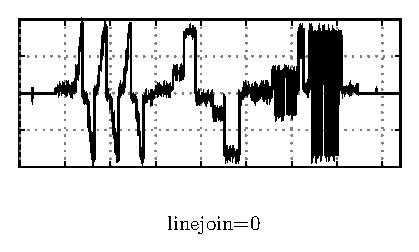
\includegraphics{fig_NoiseData_ClosedLine}
\end{minipage}
\begin{minipage}{0.48\linewidth}
	\centering
	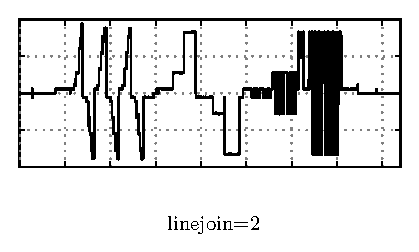
\includegraphics{fig_NoiseData_OpenLine}
\end{minipage}



\subsection{Customized Tick Labels}\label{sec:CustomTickLabels}

A common task is to plot a graph without numeric tick labels but with selected customized labels. This is easily accomplished by setting the option \verb|NoTickLabel| when plotting the axis and adding the customized labels with the commands \verb|PutTickLabelXaxis| and \verb|PutTickLabelYaxis|. Note that when setting \verb|NoTickLabel| for an axis, the option \verb|ax| has to be set in each call of \verb|PutTickLabelXaxis| and \verb|PutTickLabelYaxis| according to the axis one wishes to place the label at. This is also required if only the lower x-axis or left y-axis are plotted and tick labelled.

\begin{minipage}[T]{0.5\linewidth}
	\lstinputlisting[linerange=5-12]{examples/furtherEx_TickLabels}
\end{minipage}
\hspace{1ex}
\begin{minipage}[T]{0.4\linewidth}
	\begin{NumericDataPlot}{\textwidth}{6cm}
	\setxAxis{xMin=1, xMax=1.6, Dx=0.1, DDx=0.2}
	\setyAxis{yMin=75, yMax=130, Dy=12.5}
	
	\plotxAxis[NoTickLabel]{x-axis label}
	\plotyAxis[NoLabel, NoTickLabel]{y-axis label}
	
	\PutTickLabelXaxis[x=1.2, ax=lower]{test}
	\PutTickLabelXaxis[x=1.1, ax=upper]{test1}

	\PutTickLabelYaxis[y=80, ax=left]{test}
	\PutTickLabelYaxis[y=100, ax=right]{test1}
	
	
	\listplot[style=StdLineStyA]{\IdentI}
	\listplot[style=StdLineStyB]{\IdentII}
	
\end{NumericDataPlot}
\end{minipage}
